% Chapter 1

\chapter{Introducción general} % Main chapter title

\label{Chapter1} % For referencing the chapter elsewhere, use \ref{Chapter1} 
\label{IntroGeneral}

En el capítulo siguiente se presenta una introducción general al trabajo realizado. Se describe el problema que el \textit{Rhynchophorus Ferrugineus} (picudo rojo) presenta en las palmeras de la ciudad de Montevideo, el estado del arte en cuanto a trabajos similares y los objetivos planteados por la Intendencia de Montevideo (IM) y por el equipo de trabajo.

%--------------------------------------------------------------------------------------------------------------------------------------------------------------------------------

% Define some commands to keep the formatting separated from the content 
\newcommand{\keyword}[1]{\textbf{#1}}
\newcommand{\tabhead}[1]{\textbf{#1}}
\newcommand{\code}[1]{\texttt{#1}}
\newcommand{\file}[1]{\texttt{\bfseries#1}}
\newcommand{\option}[1]{\texttt{\itshape#1}}
\newcommand{\grados}{$^{\circ}$}
\newcommand{\comment}[1]{}

%--------------------------------------------------------------------------------------------------------------------------------------------------------------------------------
\section{Descripción del problema}
\label{sec:descProblema}

El picudo rojo, que puede observarse en la figura \ref{fig:picudo-rojo}, es un insecto que afecta a las palmeras, especialmente a la \textit{Phoenix Canariensis}, que es la especie más común en Montevideo. Este insecto ha causado un daño significativo en la flora de la ciudad, lo que ha llevado a la Intendencia de Montevideo (IM) a enfocarse en su control y erradicación.

\begin{figure}[htpb]
  \centering
  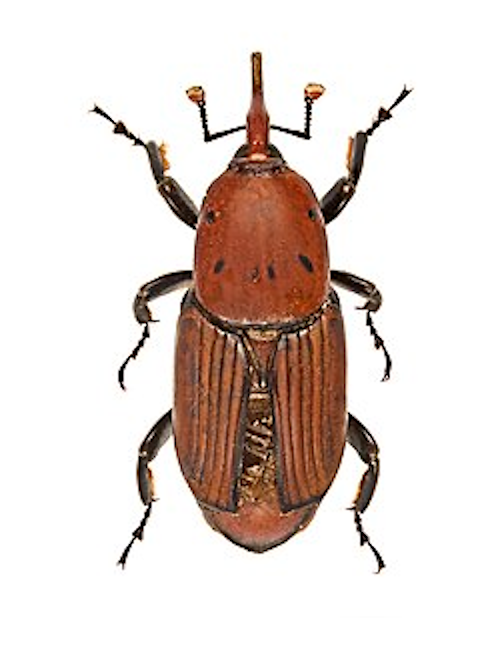
\includegraphics[scale=1]{./Figures/picudo-rojo.png}
  \caption{Picudo rojo\protect\footnotemark.}
  \label{fig:picudo-rojo}
\end{figure}

\footnotetext{Imagen tomada de \url{https://es.wikipedia.org/wiki/Rhynchophorus_ferrugineus}}

Este escarabajo supone una amenaza grave para las palmeras, ya que una vez infectada, como puede verse en la figura \ref{fig:palmera-infectada}, sus larvas se alimentan de su tejido interno, causando el colapso estructural de estas plantas en un período de meses, dado su corto ciclo de vida \citep{anticimex_picudo_nodate}. Esta amenaza aumenta según la época del año, ya que el insecto tiene diferentes tasas de dispersión y reproducción dependiendo de la temperatura y la humedad. Existen varios tipos de picudos \citep{poplin_palm_2014}, algunos autóctonos y otros introducidos.

La plaga del picudo rojo llegó al Uruguay en 2022 \citep{mgap_informacion_nodate}, esparciéndose rápidamente por la ciudad de Montevideo (de las 25.000 palmeras que forman una parte esencial de la ciudad, muchas ya han sucumbido a la plaga, donde se estima que para el año 2030 el ecosistema se verá ampliamente afectado \citep{arcos_picudo_2024}, sino se toman medidas de control adecuadas). Sin embargo, últimamente también se ha esparcido por el interior del país, como puede observarse en la figura \ref{fig:palmeras-ruta5}, perteneciente a la ruta 5 de Uruguay, donde se han encontrado palmeras muertas por la plaga.

\begin{figure}[htpb]
  \centering
  \begin{subfigure}[b]{0.49\textwidth}
    \centering
    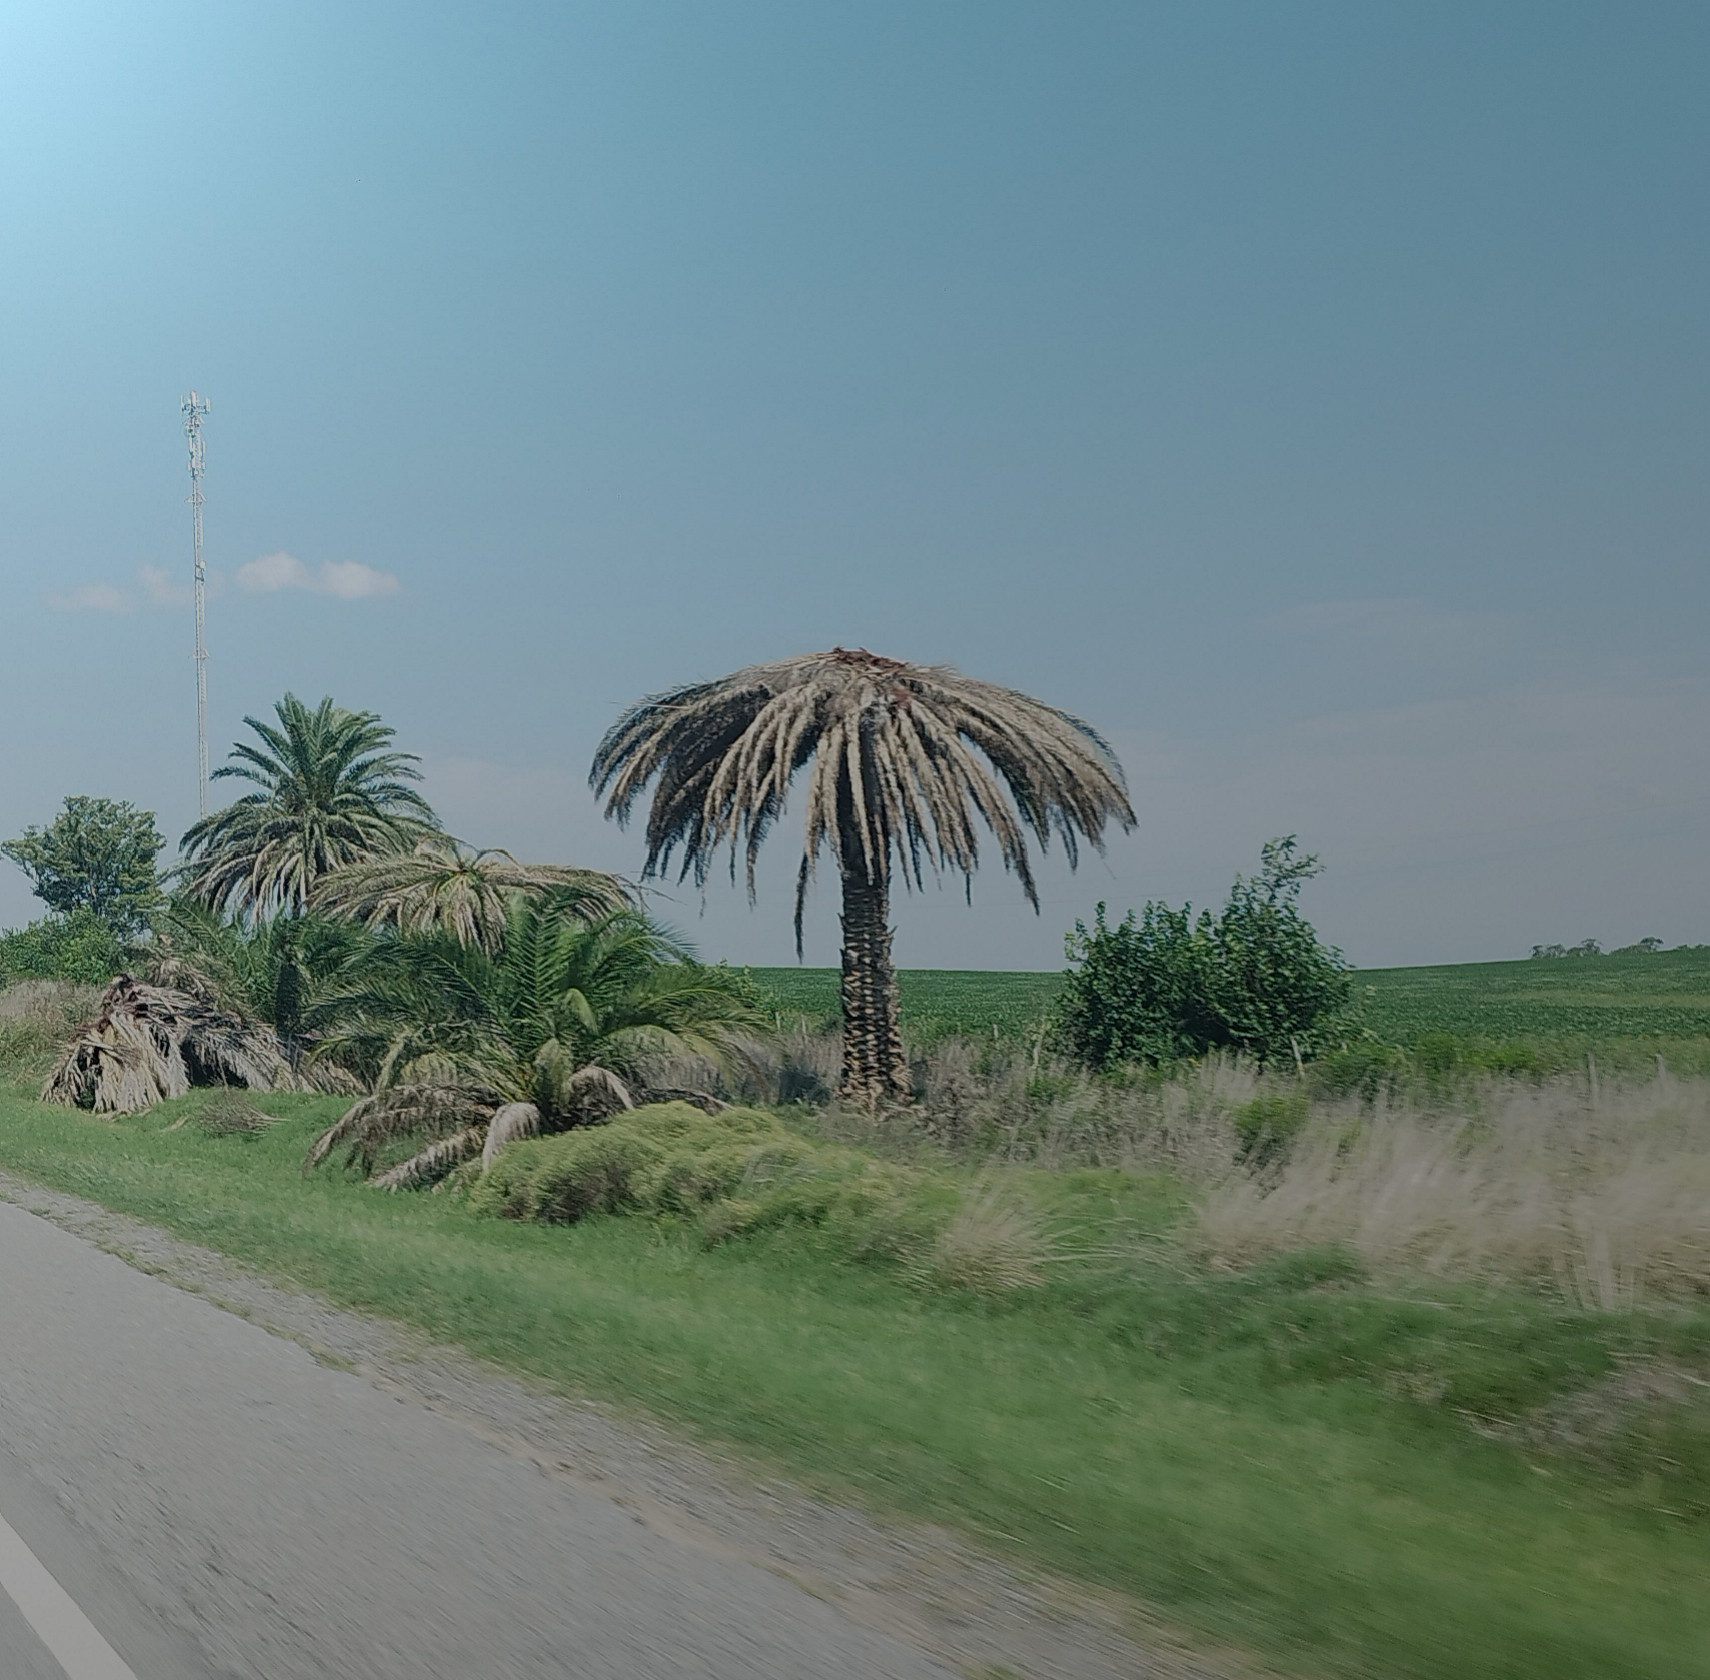
\includegraphics[width=\textwidth]{./Figures/palmera-infectada.jpg}
    \caption{Palmera infectada por el picudo rojo.}
    \label{fig:palmera-infectada}
  \end{subfigure}
  \hfill
  \begin{subfigure}[b]{0.49\textwidth}
    \centering
    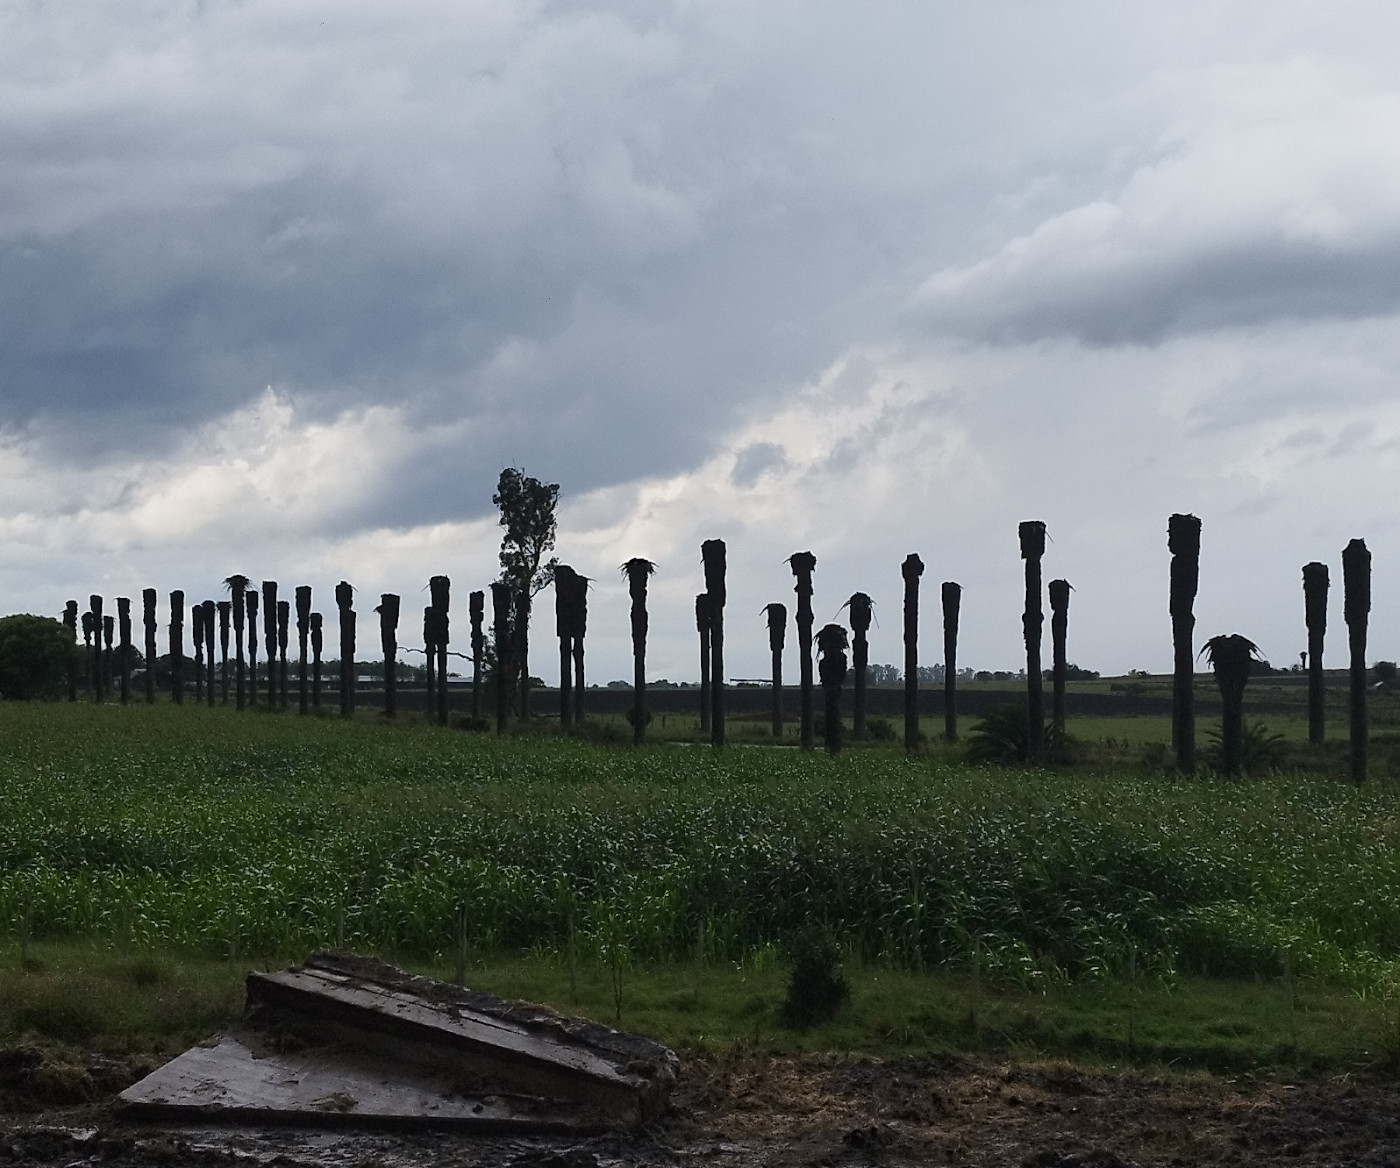
\includegraphics[width=.99\textwidth]{./Figures/palmeras-ruta5.jpg}
    \caption{Palmeras muertas en la ruta 5 de Uruguay.}
    \label{fig:palmeras-ruta5}
  \end{subfigure}
  \caption{Infección y muerte de palmeras por el picudo rojo.}
  \label{fig:infeccion-y-muerte-palmeras}
\end{figure}

Entre los métodos de control fitosanitarios que se utilizan para combatir la plaga, se encuentran: endoterapia\footnotemark, baño, cirugía\footnotemark y remoción. Sin embargo, estos métodos son costosos y requieren de un monitoreo constante para detectar la presencia del picudo rojo. Para la IM no es solamente una cuestión ecológica sino también económica. En este sentido, el servicio de Arbolado realiza un seguimiento de las palmeras afectadas por la plaga. Para ello, se registra su ubicación y estado de salud, mediante campañas de detecciones a pie. Este proceso manual requiere de mucho tiempo y recursos humanos, por lo que resulta imprescindible un sistema automatizado que permita detectar la presencia de la plaga en lugares específicos de Montevideo.

\footnotetext{Se puede obtener más información sobre la endoterapia y su aplicación por parte de la IM en \url{https://montevideo.gub.uy/noticias/urbanismo-y-obras/acciones-de-la-intendencia-de-montevideo-contra-el-picudo-rojo}}

\footnotetext{Se puede obtener más información sobre cirugías en el siguiente enlace: \url{https://www.phytoma.com/images/pdf/235_Picudo_cirugia.pdf}}

Uno de los recursos aún no explotados por la IM para el monitoreo de la plaga es el uso de imágenes aéreas obtenidas mediante drones, disponibles por el servicio de Geomática de esta institución. Estos ortomosaicos, que se puede observar un ejemplo en la figura \ref{fig:ejemplo-ortomosaico}, permiten obtener información detallada sobre el estado de las palmeras y su entorno.

\begin{figure}[H]
  \centering
  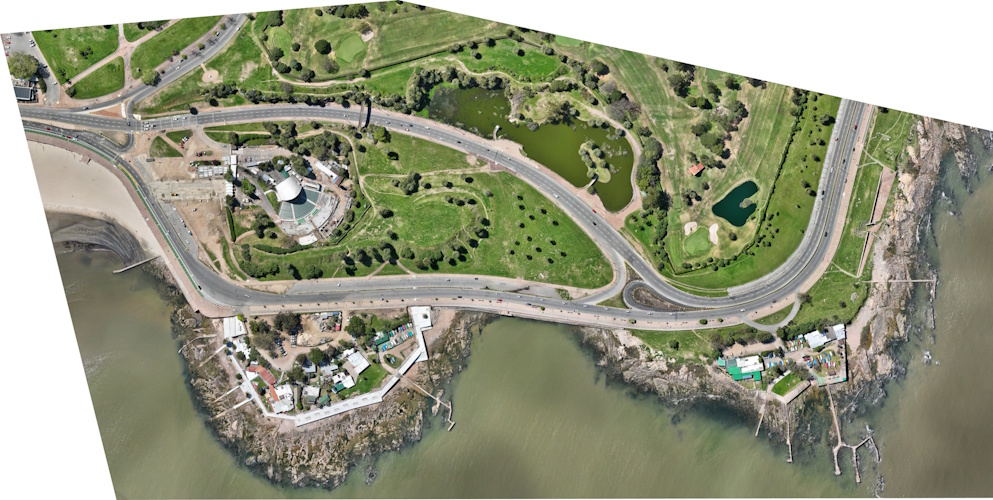
\includegraphics[scale=0.5]{./Figures/ejemplo-ortomosaico.jpg}
  \caption{Ejemplo de ortomosaico\protect\footnotemark.}
  \label{fig:ejemplo-ortomosaico}
\end{figure}

\footnotetext{Imagen tomada del sistema de información geográfica de la IM (SIG): \url{https://sig.montevideo.gub.uy/}}

El análisis de estas imágenes es un proceso complejo que requiere de técnicas avanzadas de procesamiento de imágenes y aprendizaje automático, así como también herramientas que brinden soporte a estas actividades.

%--------------------------------------------------------------------------------------------------------------------------------------------------------------------------------
\section{Estado del arte}
\label{sec:estadoArte}

\subsection{Redes convolucionales}
\label{sec:redesConvolucionales}

Visión por computadora se define como el proceso mediante el cual se extrae, analiza y comprende información significativa a partir de imágenes o secuencias de imágenes \citep{bmva_what_2017}. Este proceso abarca una amplia gama de tareas, tales como la detección de objetos, la segmentación de imágenes, el reconocimiento de patrones y la clasificación de imágenes. Dentro del ámbito de la inteligencia artificial, visión por computadora se reconoce como un subcampo destinado a dotar a las máquinas de la capacidad de interpretar y comprender la información visual del entorno de manera análoga a la percepción humana \citep{torralba_foundations_2024}. Asimismo, esta tecnología ha adquirido un papel preponderante en diversas industrias, al contribuir de forma significativa a la optimización de la eficiencia operativa y a la mejora de los procesos de toma de decisiones.

El notable desarrollo de la visión por computadora ha sido posible gracias a los avances en el campo del aprendizaje automático, en particular mediante la adopción de metodologías de aprendizaje profundo. Estas técnicas han permitido realizar importantes descubrimientos en el reconocimiento y procesamiento de imágenes, generando aplicaciones concretas en el mundo real \citep{dong_applications_2024}.

Desde la introducción de las técnicas de aprendizaje profundo a comienzos de la década de 2010, y especialmente con el surgimiento de las redes neuronales convolucionales (CNN), tanto la investigación como la aplicación práctica de la visión por computadora han experimentado transformaciones significativas. El hito representado por \textit{AlexNet} en la competición \textit{ImageNet} de 2012 \citep{krizhevsky_imagenet_2017}, así como el desarrollo de arquitecturas modernas como \textit{You Only Look Once} (YOLO) \cite{redmon_you_2016}, ejemplifican este progreso.

Las redes neuronales convolucionales constituyen una clase de modelos de aprendizaje profundo específicamente diseñados para el procesamiento y análisis de datos visuales. Estas redes se caracterizan por una arquitectura compuesta por capas convolucionales, capas de \textit{pooling} y capas densas (\textit{fully connected}), lo que les confiere la capacidad de detectar y aprender características jerárquicas presentes en las imágenes de entrada. Una representación típica de la arquitectura de estas redes se ilustra en la figura \ref{fig:vgg}.

\begin{figure}[htpb]
  \centering
  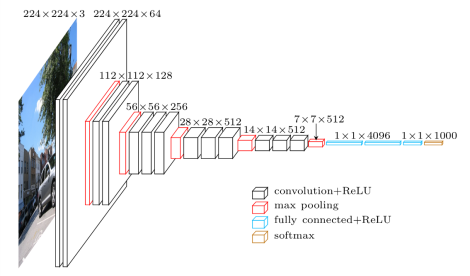
\includegraphics[scale=0.8]{./Figures/vgg.png}
  \caption{Red convolucional VGG\protect\footnotemark.}
  \label{fig:vgg}
\end{figure}

\footnotetext{Imagen obtenida de: \url{https://paperswithcode.com/method/vgg}}

Las tendencias recientes en el ámbito de las redes neuronales convolucionales (CNN) evidencian avances significativos en el diseño de sus arquitecturas y en el procesamiento de datos, orientados a la solución de problemáticas emergentes. En particular, se ha puesto especial énfasis en el tratamiento de imágenes de alta resolución capturadas mediante vehículos aéreos no tripulados, tales como drones, lo que representa un área de aplicación de creciente interés académico y práctico \citep{gao_recent_2024} \citep{sutar_convolutional_2025}.

\subsection{Detección del picudo rojo en imágenes aéreas}

La relevancia de la detección de la plaga del picudo rojo a nivel global ha propiciado el surgimiento de diversas líneas de investigación. En este sentido, se han desarrollado enfoques basados en visión por computadora a partir de imágenes aéreas, haciendo especial uso de arquitecturas de redes neuronales convolucionales (CNN) descritas en la sección \ref{sec:redesConvolucionales}.

Entre los estudios analizados, la implementación de la detección mediante imágenes aéreas de forma exclusiva representa una metodología relativamente novedosa. En este contexto, en el estudio "\textit{Automatic large scale detection of red palm weevil infestation using street view images} \citep{kagan_automatic_2021}", se emplea un enfoque combinado. Inicialmente, se localizan las palmas a través de una CNN (Faster R-CNN \citep{ren_faster_2016}) aplicada a imágenes aéreas. Posteriormente, utilizando la misma arquitectura, se extrae la corona de la palmera a partir de imágenes capturadas en \textit{street view}, permitiendo clasificar a la planta en función de la presencia o ausencia de infección. Un resumen de este trabajo se presenta en la figura \ref{fig:kagan-automatic-2021-process}.

\begin{figure}[htpb]
  \centering
  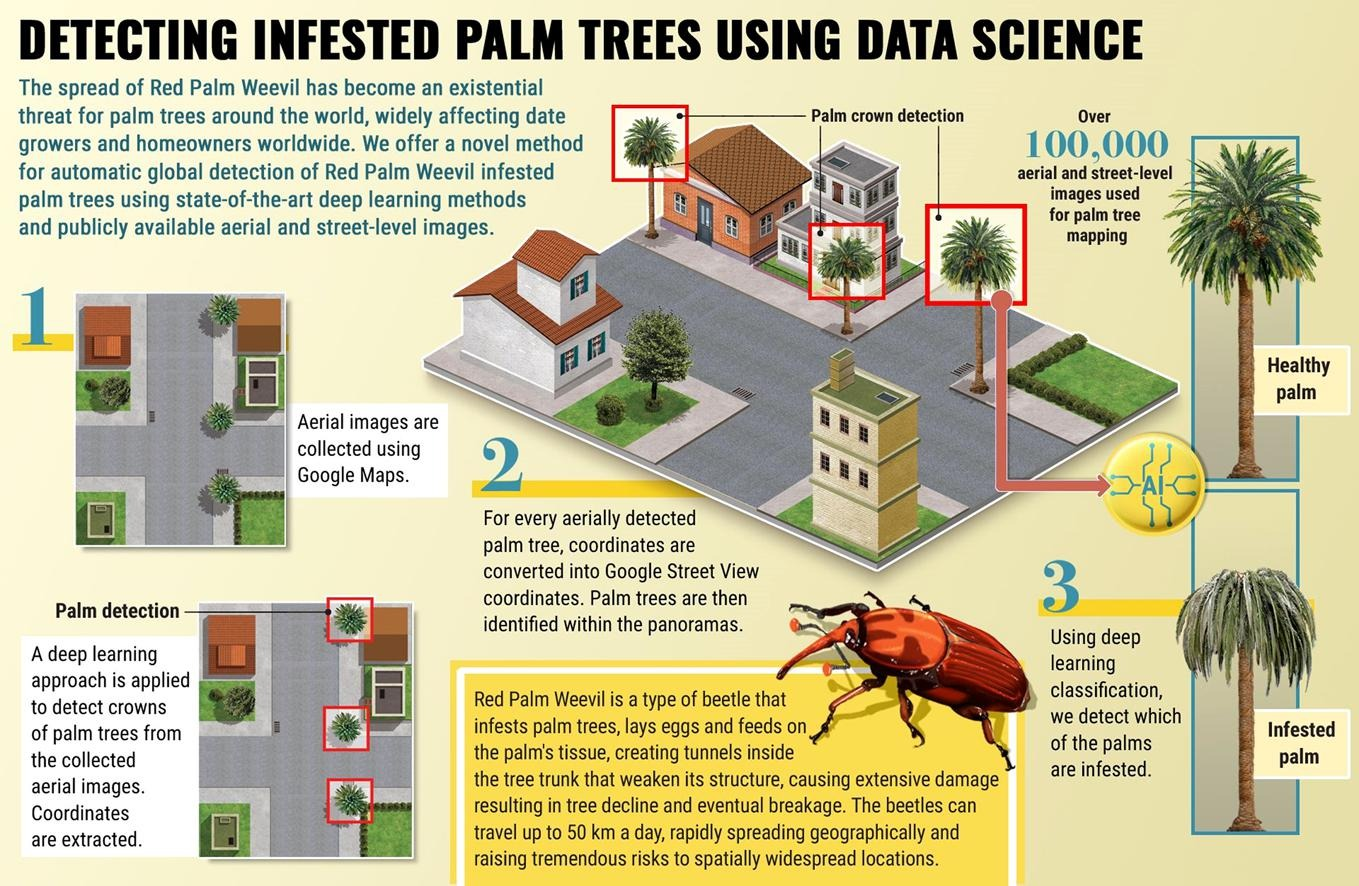
\includegraphics[scale=1.8]{./Figures/kagan_automatic_2021-process.jpg}
  \caption{Proceso de detección realizado por Kagan et al\protect\footnotemark.}
  \label{fig:kagan-automatic-2021-process}
\end{figure}

\footnotetext{Imagen obtenida de: \url{http://arxiv.org/abs/1506.01497}}

La detección de palmeras sí es ampliamente estudiada en la literatura, siendo un tema recurrente en la investigación de visión por computadora. En este sentido, se han desarrollado diversos estudios. En "\textit{Implementation of slicing aided hyper inference (SAHI) in YOLOv8 to counting oul palm trees using high-resolution aereal imagery data} \citep{zhorif_implementation_2024}" se presenta un enfoque que utiliza la arquitectura YOLOv8 para detectar palmeras en imágenes aéreas de alta resolución. Además, utiliza \textit{Slicing Aided Hyper Inference} (SAHI) para mejorar la precisión de la detección. Este enfoque se basa en la idea de dividir las imágenes en regiones más pequeñas y realizar inferencias en cada una de ellas, lo que permite una detección más precisa de los objetos de interés, especial en el caso de objetos pequeños como las palmeras. Para el estudio, se utilizaron imágenes RGB capturadas con un dron Trinity F90+ a 200 metros de altura y una implementación de segmentación (SAHI) de unos 3000x3000 píxeles. Si bien el estudio se centra en la detección de palmeras de aceite, su metodología puede ser adaptada para la detección del picudo rojo. Se destaca la tabla \ref{tab:papers-deteccion-palmeras} que resume los métodos utilizados en la detección de palmeras en diferentes estudios anteriores.

\begin{table}[H]
  \centering
  \caption[comparativa-papers]{Comparación entre diferentes estudios de detección de palmeras\footnotemark.}
  \begin{tabular}{{l c c}}
    % \begin{tabular}{{l p{4cm} p{4cm}}}
    \toprule
    \textbf{Autor y año}                                          & \textbf{Modelo}       & \textbf{Métricas}               \\
    \midrule
    Mukhles Sir Monea et al, 2022\citep{muna_development_2023}        & YOLOv3                & 5.76\% (MAPE)                     \\
    Hery Wibowo et al, 2022\citep{wibowo_large-scale_2022}            & \makecell[c]{YOLOv3,                                      \\YOLOv4, \\YOLOv5m}            & \makecell[c]{97.28\% (v3), \\97.74\% (v4), \\94.94\% (v5m). \\(F1-Score)}              \\
    Adel Ammar et al, 2022\citep{ammar_deep-learning-based_2021}      & Faster R-CNN          & \makecell[c]{94.99\% (Precision), \\84\% (Recall), \\83\% (AP IoU)}                 \\
    Wardana et al, 2023\citep{wardana_detection_2023}                 & YOLOv8                & 98.50\% (Overall Accuracy)        \\
    Deta Sandya Prasitha et al, 2022\citep{prasvita_automatic_nodate} & \makecell[c]{YOLOv5s,                                     \\YOLOv5m, \\YOLOv5l, \\YOLOv5x} & \makecell[c]{0.82 (v5s), \\0.84 (v5m), \\0.85 (v5l), \\0.86 (v5x). \\(Average F1-Score)} \\
    Nuwar et al, 2022\citep{nuwara_modern_2022}                       & YOLOv5                & 0.895 (F1-Score)                  \\
    Junos et al, 2022\citep{junos_notitle_nodate}                     & YOLOv3n               & \makecell[c]{97.20\% (mAP),       \\0.91 (F1-Score)}                                     \\
    \bottomrule
    \hline
  \end{tabular}
  \label{tab:papers-deteccion-palmeras}
\end{table}

% \begin{table}[h]
%   \centering
%   \caption[comparativa-papers]{Comparación entre diferentes estudios de detección de palmeras\footnotemark.}
%   \begin{adjustbox}{width=\textwidth}
%     \begin{tabular}{l c c}
%       \toprule
%       \textbf{Author and Year}         & \textbf{Method}                    & \textbf{Evaluation}                                                \\
%       \midrule
%       Mukhles Sir Monea et al, 2022    & YOLOv3                             & 5.76\% (MAPE)                                                      \\
%       Hery Wibowo et al, 2022          & YOLOv3, YOLOv4, YOLOv5m            & 97.28\% (v3), 97.74\% (v4), 94.94\% (v5m). (F1-Score)              \\
%       Adel Ammar et al, 2022           & Faster R-CNN                       & 94.99\% (Precision), 84\% (Recall), 83\% (AP IoU)                  \\
%       Wardana et al, 2023              & YOLOv8                             & 98.50\% (Overall Accuracy)                                         \\
%       Deta Sandya Prasitha et al, 2022 & YOLOv5s, YOLOv5m, YOLOv5l, YOLOv5x & 0.82 (v5s), 0.84 (v5m), 0.85 (v5l), 0.86 (v5x). (Average F1-Score) \\
%       Nuwar et al, 2022                & YOLOv5                             & 0.895 (F1-Score)                                                   \\
%       Junos et al, 2022                & YOLOv3n                            & 97.20\% (mAP), 0.91 (F1-Score)                                     \\
%       \bottomrule
%       \hline
%     \end{tabular}
%   \end{adjustbox}
%   \label{}
% \end{table}

\footnotetext{Tabla obtenida de \textit{Implementation of slicing aided hyper inference (SAHI) in YOLOv8 to counting oul palm trees using high-resolution aereal imagery data} \citep{zhorif_implementation_2024}}

También se han realizado estudios controlados como en "\textit{Red Palm Weevil Detection in Date Palm Using Temporal UAV Imagery} \citep{delalieux_red_2023}", en donde se concluye que la detección del picudo rojo puede ser posible mediante imágenes aéreas en el rango infrarrojo.

%--------------------------------------------------------------------------------------------------------------------------------------------------------------------------------

\section{Objetivos y alcance}
\label{sec:objetivos}

La finalidad principal del presente trabajo consistió en validar una prueba de concepto para la detección del picudo rojo en palmeras de Montevideo, utilizando imágenes aéreas capturadas mediante drones. Con este objetivo, se desarrolló un sistema fundamentado en técnicas de visión por computadora y aprendizaje profundo, el cual permite identificar la presencia de la plaga. Para ello, se empleó el SIG\footnotemark, complementado con herramientas adicionales que facilitaron la generación del conjunto de datos de entrenamiento.

\footnotetext{El SIG de la IM se encuentra disponible en \url{https://sig.montevideo.gub.uy/}}

Adicionalmente, se planteó ante la intendencia de Montevideo la necesidad de optimizar los procesos de detección de la plaga, con miras a una mejora en la asignación de recursos humanos y económicos. El alcance inicial se centró exclusivamente en la detección del picudo rojo, y en los capítulos siguientes se detalla tanto la descripción de las herramientas utilizadas como el proceso metodológico implementado.

% Objetivos para la intendencia de Montevideo y objetivos técnicos. Alcance: anotaciones y modelado.